\section{eo\-External\-Quad\-Op$<$ F, External, External\-EO $>$ Class Template Reference}
\label{classeo_external_quad_op}\index{eoExternalQuadOp@{eoExternalQuadOp}}
Crossover of external struct, ctor expects a function of the following signature:.  


{\tt \#include $<$eo\-External\-Op\-Functions.h$>$}

Inheritance diagram for eo\-External\-Quad\-Op$<$ F, External, External\-EO $>$::\begin{figure}[H]
\begin{center}
\leavevmode
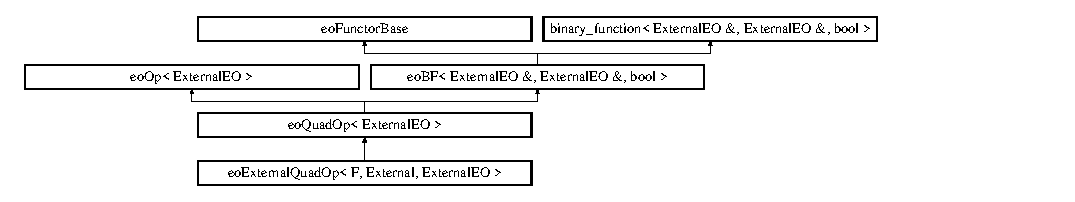
\includegraphics[height=2.26263cm]{classeo_external_quad_op}
\end{center}
\end{figure}
\subsection*{Public Member Functions}
\begin{CompactItemize}
\item 
{\bf eo\-External\-Quad\-Op} (bool($\ast$\_\-quadop)(External \&, External \&))\label{classeo_external_quad_op_a0}

\item 
bool {\bf operator()} (External\-EO \&eo1, External\-EO \&eo2)\label{classeo_external_quad_op_a1}

\begin{CompactList}\small\item\em The pure virtual function that needs to be implemented by the subclass. \item\end{CompactList}\end{CompactItemize}
\subsection*{Private Attributes}
\begin{CompactItemize}
\item 
bool($\ast$ {\bf quadop} )(External \&, External \&)\label{classeo_external_quad_op_r0}

\end{CompactItemize}


\subsection{Detailed Description}
\subsubsection*{template$<$class F, class External, class External\-EO = eo\-External\-EO$<$F, External$>$$>$ class eo\-External\-Quad\-Op$<$ F, External, External\-EO $>$}

Crossover of external struct, ctor expects a function of the following signature:. 

bool func(External\&, External\&);

Where External is the user defined struct or class The function should return true when it changed something, false otherwise 



Definition at line 154 of file eo\-External\-Op\-Functions.h.

The documentation for this class was generated from the following file:\begin{CompactItemize}
\item 
eo\-External\-Op\-Functions.h\end{CompactItemize}
